%% SECTION HEADER /////////////////////////////////////////////////////////////////////////////////////
\section{Displacements Coupling at the Interface of Substructures}
\label{sec:interface}

%% SECTION CONTENT ////////////////////////////////////////////////////////////////////////////////////

The present model of the sandwich panel consists of \ac{2d} and \ac{3d} elements. 
Moreover, there are non-matching grids between two adjacent substructures. 
These involve connecting them by imposing the compatibility of the displacements at the interface, see Fig.~\ref{fig:interface}.
This type of connection is implemented through the interface elements based on Lagrange multipliers, which are interpreted as forces responsible for determining the appropriate displacements of nodes.
The coupling can be expressed as:
\begin{eqnarray}
	\left\{\begin{array}{c}
		\textbf{u}\\
		\textbf{v}\\
		\textbf{w}
	\end{array}\right\}_{s_{i1}}^{\Gamma^i}-
	\left\{\begin{array}{c}
		\textbf{u}\\
		\textbf{v}\\
		\textbf{w}
	\end{array}\right\}_{s_{i2}}^{\Gamma^i}=
	\left\{\begin{array}{c}
		\textbf{0}\\
		\textbf{0}\\
		\textbf{0}
	\end{array}\right\},
	\label{eq:coupling}
\end{eqnarray}
\begin{figure}
	\begin{center}
		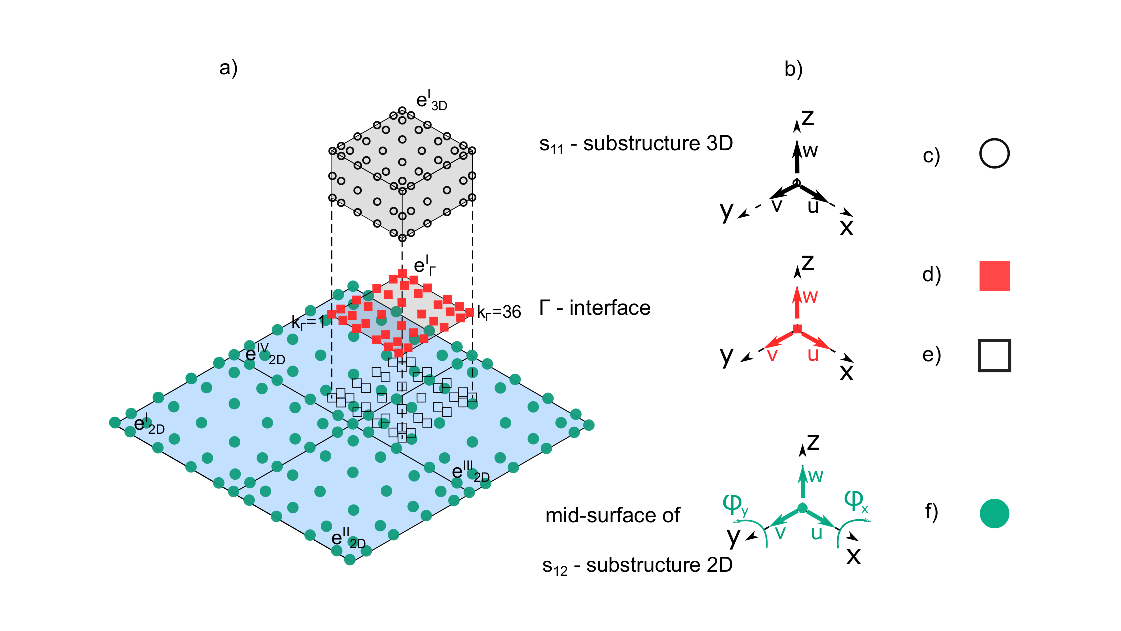
\includegraphics[scale=0.8]{Chapter_4/interface_2D3D}
	\end{center}
	\caption{Non-matching interface setup: a) interface coupling, b) degrees-of-freedom of the interface and the substructures.}
	\label{fig:interface}
\end{figure}
where \(s_{i1}\) and \(s_{i2}\) are substructures connected by the interface \(\Gamma^i\). For the whole structure, the Eq.~(\ref{eq:coupling}) can be written in the matrix form:
\begin{eqnarray}
	\textbf{G}\textbf{d}=\textbf{0},
	\label{eq:cond_disp}
\end{eqnarray}
where \textbf{G} is the coupling matrix which contains the equations to interpolate the substructures displacements at the interfaces, and \(\textbf{d}\) is a global displacement field for \(nS\) number of substructures, composed as:
\begin{eqnarray}
	\textbf{d} = \left\{\begin{array}{cccc}
		\textbf{d}_1, & \textbf{d}_2, &\ldots, & \textbf{d}_{nS}
	\end{array}\right\}^T.
	\label{eq:displacements}
\end{eqnarray}

General formulation of the matrix \textbf{G} is presented in Algorithm \ref{alg:G_matrix}.

\begin{algorithm}[H]
	\SetAlgoLined
	\KwResult{coupling matrix \textbf{G}}
	\For{i = 1 \KwTo 2}{
		create \(n^{\Gamma}\times n^{s_i}\) null matrix 
		\(\mathbf{G}_i\),\\
		\For{j = 1 \KwTo \(n^{\Gamma}\)} {
			find \(ownerElement^j_i\) in the structure \(s_i\) 
			containing interface node \(j\) with global coordinates vector: 
			\(X_p=(x^j_p,y^j_p)\)\;
			assign vector \(X_e=(x_e,y_e)\) of coordinates of all nodes in 
			\(ownerElement^j_i\)\;
			assign initial coordinates 
			\(X_{\kappa}=(x^j_{\kappa},y^j_{\kappa})\) to the nearest node in
			\(ownerElement^j_i\) to node \(j\)\;
			transform global coordinates \(X_{\kappa}\) to a local coordinate system \(\xi_{\kappa}=\xi(X_{\kappa});\quad 
			\eta_{\kappa}=\eta(X_{\kappa})\)\;
			\While{\(\left|X_p-X_{\kappa}\right|>tol\)}{
				\(\xi_{\kappa+1}=\xi_{\kappa}+(J^{-1}_{\kappa})_{11}.*(x^j_p-x_{\kappa}^j)
				+(J^{-1}_{\kappa})_{12}.*(y^j_p-y_{\kappa}^j)\)\;
				\(\eta_{\kappa+1}=\eta_{\kappa}+(J^{-1}_{\kappa})_{21}.*(x^j_p-x_{\kappa}^j)
				+(J^{-1}_{\kappa})_{22}.*(y^j_p-y_{\kappa}^j)\)\;
				\(X_{\kappa}=N_{\kappa+1}X_e\)\;
			}
			\(\mathbf{G}_i(j,n^{X_e})=N_{\kappa+1}\)\;
		}
		\uIf{\(s_i\) is 3D} {
			\(\mathbf{G}_i=\left[\begin{array}{ccc}
				\mathbf{G}_i & \mathbf{0} & \mathbf{0}\\
				\mathbf{0} & \mathbf{G}_i & \mathbf{0}\\
				\mathbf{0} & \mathbf{0} & \mathbf{G}_i
			\end{array} \right]
			\)\;
		}
		\ElseIf{\(s_i\) is 2D} {
			\(\mathbf{G}_i=\left[\begin{array}{ccccc}
				\mathbf{G}_i & \mathbf{0} & \mathbf{0} & 
				\frac{h_i}{2}\mathbf{G}_i & \mathbf{0}\\
				\mathbf{0} & \mathbf{G}_i & \mathbf{0} & \mathbf{0} & 
				\frac{h_i}{2}\mathbf{G}_i\\
				\mathbf{0} & \mathbf{0} & \mathbf{G}_i & \mathbf{0} & 
				\mathbf{0}
			\end{array} \right]\)\;
		}
	}
	\(\mathbf{G}=\left[\begin{array}{cc}
		\mathbf{G}_1 & \mathbf{G}_2
	\end{array} \right].\)
	\caption{Interface coupling matrix formulation}
	\label{alg:G_matrix}
\end{algorithm}
where \(s_i\) is the structure to, \(n^{\Gamma}\) and \(n^{s_i}\) are numbers of nodes of the interface, respectively; \(J_{\kappa}\) is the Jacobian evaluated at \((\xi_{\kappa},\eta_{\kappa})\) and \(N_{\kappa+1}\) is the shape function evaluated at \((\xi_{\kappa+1},\eta_{\kappa+1})\), \(n^{X_e}\) is the vector of global order numbers of all nodes in the \(ownerElements^j_i\), \(h_i\) is a thickness of the structure \(s_i\) and \(tol\) is a termination criterion for iterations.

The main task of the algorithm is to calculate shape functions for each adjacent substructures at the points \(X_p=(x_p^k,y_p^k)\), which are projections of the interface nodes onto these substructures.
The shape function can be calculated after finding an owner element and local coordinates of the points.
Owner element is a spectral element in the domain of the substructure \(s_{ij}\) which contains interface node, for example, interface node \(k_\Gamma=36\) (see~Fig.~\ref{fig:interface}a)) is located in the element \(e^{I}_{3D}\) and \(e^{III}_{2D}\) for the substructures \(s_{11}\) and \(s_{12}\), respectively.
It can be found within two ways: using Matlab's built-in function \verb+inpolygon+ or more efficient procedure proposed by Silva et al. \cite{silva2009exact} which was used in the current implementation.
The transformation from global to local coordinates was realized by the iterative method presented in the work of Li et al.~\cite{li2014efficient}.
The computational effectiveness of Algorithm~\ref{alg:G_matrix} can be easily improved if certain precautions are taken.
Firstly, the mesh of the interface has to be based on the mesh from one of the substructures \(s_{i1}\), \(s_{i2}\), which may be referred to as a slave.
So, the shape function takes only the values of one and zeros.
Moreover, the code can be implemented in vectorized form rather than using a for-loops.